\section{Codificador de Prioridade 8x3 (Expansão)}

\subsection{Expressões Booleanas e Esquemático do Bloco H}
A decomposição utiliza os módulos 4x2 projetados anteriormente. O Bloco H atua como a lógica combinacional de união.
\subsection*{a. Expressões Booleanas do Bloco H}

Para o projeto do \textbf{Bloco H}, que atua como o estágio combinacional de junção para formar o codificador de prioridade 8x3 a partir de dois codificadores 4x2, as expressões booleanas são deduzidas analisando a precedência lógica do bloco superior.

Seja o bloco inferior responsável pelas entradas de menor peso, $x_0$ a $x_3$ (gerando os sinais $A^1, y_1^1, y_0^1$), e o bloco superior responsável pelas entradas de maior peso, $x_4$ a $x_7$ (gerando os sinais $A^2, y_1^2, y_0^2$). As expressões de saída são definidas da seguinte forma:


\textbf{Sinal de Validação Geral ($A$):} O circuito total é validado (nível lógico alto) se qualquer um dos blocos menores identificar uma entrada ativa.
    \begin{equation}
        A = A^1 + A^2
    \end{equation}

\textbf{Bit Mais Significativo ($y_2$):} Este bit indica se a entrada ativada pertence à metade superior do barramento ($x_4$ a $x_7$, correspondentes aos binários de $100_2$ a $111_2$). Logo, ele é ativado diretamente pelo sinal de validação do bloco superior.
    \begin{equation}
        y_2 = A^2
    \end{equation}

\textbf{Bits Menos Significativos ($y_1$ e $y_0$):} Para estas saídas, o Bloco H atua de forma análoga a um multiplexador controlado pelo sinal de prioridade $A^2$. Se o bloco superior possuir uma entrada ativa ($A^2 = 1$), suas saídas repassam os valores aos bits inferiores. Caso contrário ($A^2 = 0$), os bits assumem os valores repassados pelo bloco inferior. Considerando que $y_i^2$ é $0$ quando $A^2 = 0$, as equações otimizadas são:
    \begin{align}
        y_1 &= y_1^2 + (\overline{A^2} \cdot y_1^1) \\
        y_0 &= y_0^2 + (\overline{A^2} \cdot y_0^1)
    \end{align}

\begin{figure}[H]
    \centering
    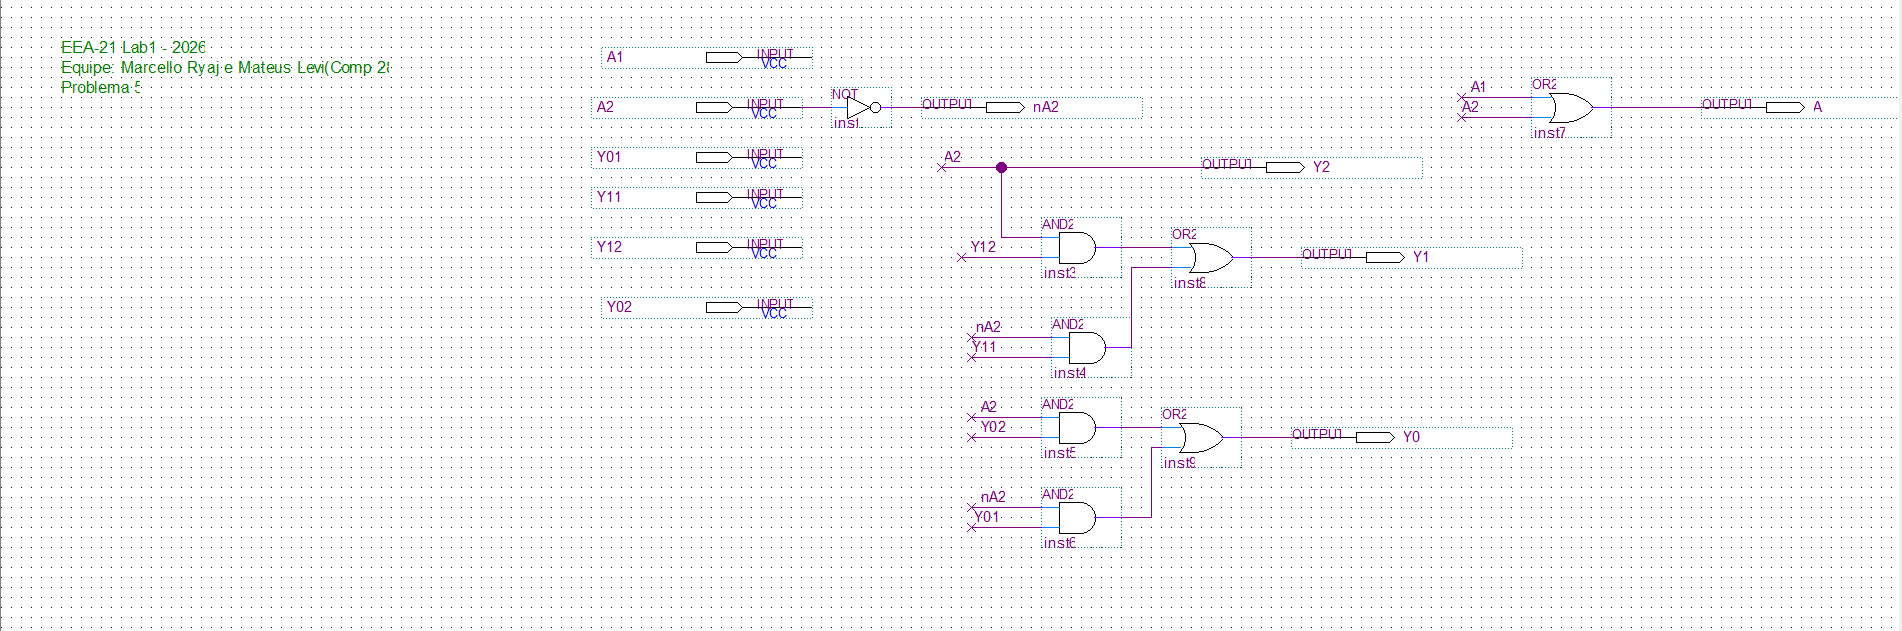
\includegraphics[width=1\textwidth]{fig/EsquematicoExercicio5.png}
    \caption{Diagrama esquemático do Bloco H.}

\end{figure}

\subsection{Diagrama de Temporização do Bloco H}

\begin{figure}[H]
    \centering
    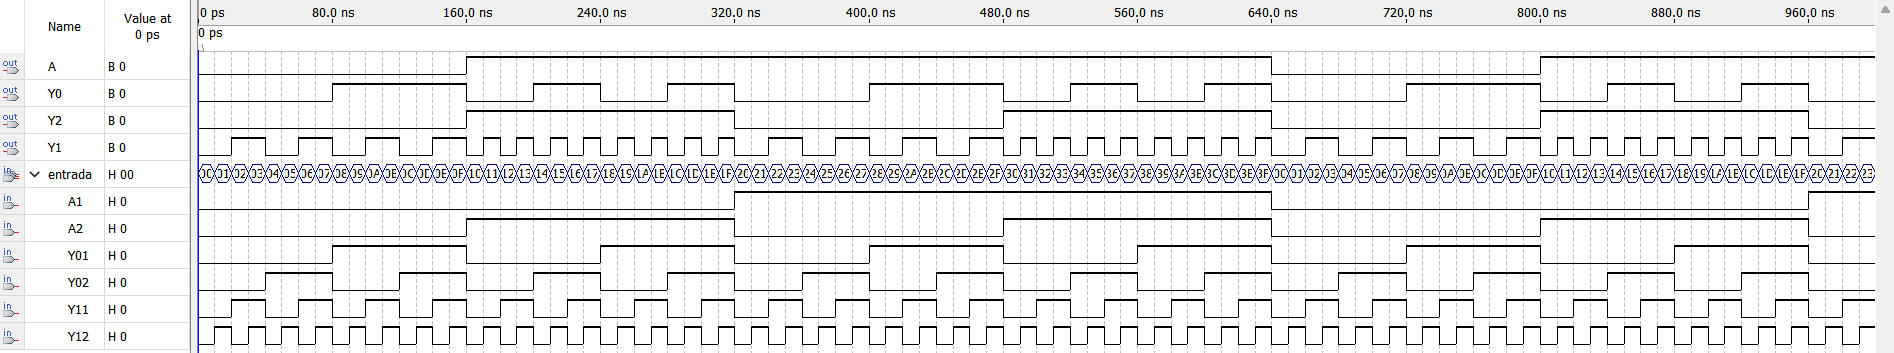
\includegraphics[width=1\textwidth]{fig/SimuExercicio5B.png}
    \caption{Simulação funcional (diagrama de temporização) do Bloco H.}

\end{figure}

A simulação apresentada na Figura 14 comprova o funcionamento do Bloco H como o estágio decisório do sistema. O diagrama atesta que o bit mais significativo ($Y_2$) e as saídas de dados ($Y_1$ e $Y_0$) replicam estritamente os valores do bloco superior sempre que sua validação ($A_2$) está ativa. Na ausência de sinal superior ($A_2 = 0$), o circuito comuta perfeitamente a lógica, repassando os dados do bloco inferior à saída final.

\subsection{Diagrama de Temporização do Dispositivo Completo}

\begin{figure}[H]
    \centering
    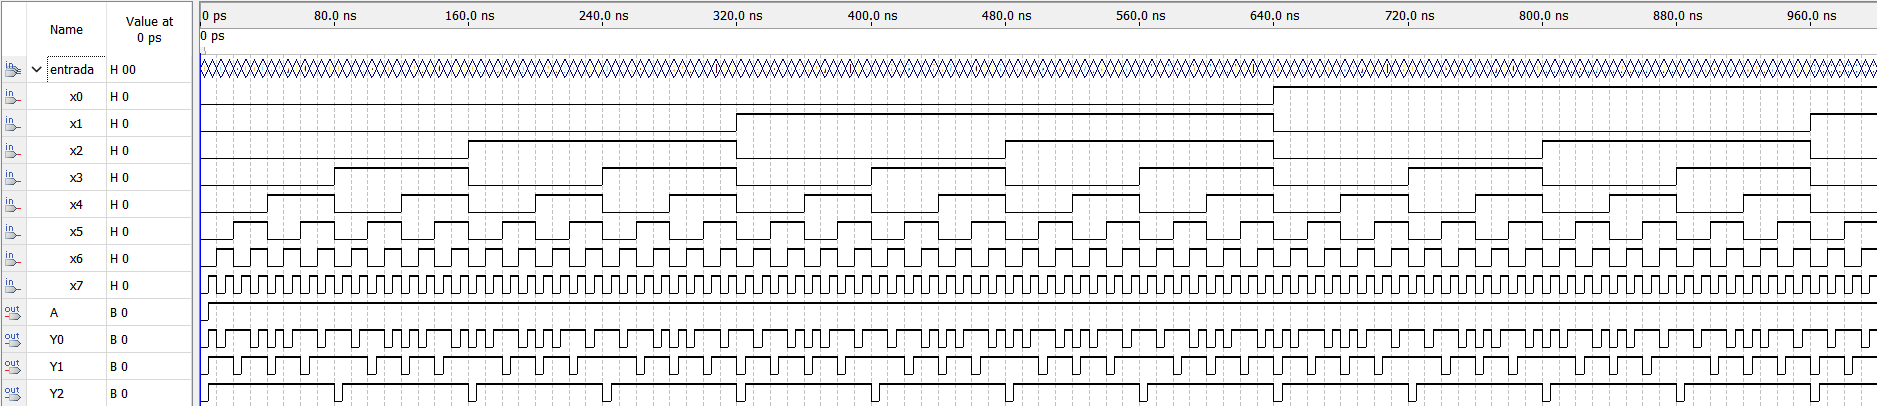
\includegraphics[width=1\textwidth]{fig/SimuExercicio5C.png}
    \caption{Simulação funcional (diagrama de temporização) do Dispositivo Completo.}

\end{figure}

A Figura 15 atesta o sucesso da integração do codificador de prioridade 8x3 (Top-Level). A análise das formas de onda demonstra a obediência incontestável à regra de precedência lógica: o barramento de saída codifica invariavelmente o valor binário da entrada ativa de maior índice (de $x_7$ a $x_0$), ignorando as entradas de menor peso. Adicionalmente, o bit de validação ($A$) opera de forma exata, acusando nível lógico baixo exclusivamente quando todas as entradas são nulas.